% Sections 6.2 to 6.4 of the revised paper (real model outputs, window robustness, ablation reading). Numbers come from numbers_generated.tex.

\subsection{Real model outputs}\label{sec:res-real}

We ran three open models on CPU and recorded their outputs (Section~\ref{sec:protocol}): Qwen2.5-1.5B-Instruct for MMLU and TruthfulQA, GPT-2 for RealToxicityPrompts, and Qwen2.5-0.5B for the replication. The risk is $1-p(\text{correct})$ for the two question-answering tasks and the toxicity probability of a continuation for the third. The tasks differ in one way that matters for this paper: how much the \emph{upper tail} of the risk moves between regimes, because the threshold $q_t$ targets the $0.9$ quantile.

\paragraph{MMLU and TruthfulQA: the upper tail does not move.}
Qwen2.5-1.5B-Instruct answers \MmluAcc{} of the \MmluN{} MMLU questions correctly. Across the four broad categories the median risk moves a great deal (from \MmluMedLo{} to \MmluMedHi{}) but the $0.9$ quantile does not (\MmluQnineLo{} to \MmluQnineHi{}). A threshold at the $0.9$ quantile is therefore close to $1$ in every regime, and the methods tie (Table~\ref{tab:mmlu_catblock}). In the category-block orderings static calibration already has post-shift violation \MmluCatStaticPost{}, against \MmluCatPSPost{} for PromptShift-CRC and \MmluCatMatchedPost{} for matched Adaptive CRC; the mean thresholds of the online methods lie within $0.015$ of one another; and the intervention rate is $0.999$ or higher for every method, so the decision rule never lets the model answer. PromptShift-CRC minus matched Adaptive CRC is \MmluCatPSvsMatchedPost{} (SE \MmluCatPSvsMatchedPostSE{}) in post-shift violation. The frontier gaps are \MmluCatFrontierPS{} (SE \MmluCatFrontierPSSE{}) for PromptShift-CRC and \MmluCatFrontierDtACI{} (SE \MmluCatFrontierDtACISE{}) for DtACI in the category-block orderings, and \MmluSubjFrontierPS{} and \MmluSubjFrontierDtACI{} in the subject-block orderings. On TruthfulQA the model answers \TqaAcc{} of the questions correctly under multiple-choice scoring, the $0.9$ quantile of the risk is \TqaQnine{}, and the same holds. These two tasks test the guarantee (every online method reaches the target) but not the weighting, because no weighting can help when the quantity being estimated barely changes. We report them so that the reader can see the setting in which drift-awareness has nothing to offer.

\paragraph{RealToxicityPrompts: the upper tail moves.}
We drew \RtpN{} prompts, continued each with GPT-2 (one nucleus sample of $20$ tokens), and scored the continuation with a public toxicity classifier. Only \RtpFracHigh{} of the continuations have risk above $0.5$, and they are concentrated in prompts that are themselves toxic. Split by quartiles of the prompt toxicity annotation, the $0.9$ quantile of the risk is \RtpQnineLo{} in the lowest band and \RtpQnineHi{} in the highest, so a change of band is a real shift of the target quantile. The ordering uses only the annotation of the prompt, not the model's output. In the three lowest bands the $0.9$ quantile lies below $0.06$, close to the classifier's noise floor, so the intervention rate at $\tau=0.5$ carries little information on this task and we do not interpret it.

Static calibration fails here (coverage \RtpStaticCov{}, post-shift violation \RtpStaticPost{}), and rolling calibration is better but still above target after shifts (\RtpRollingPost{}). All online methods reach the target coverage (Table~\ref{tab:rtp_bandblock}, Figure~\ref{fig:frontier-rtp}). Among them the differences are small. Post-shift violation is \RtpPSPost{} for PromptShift-CRC, \RtpMatchedPost{} for the matched baseline, \RtpAdaptWPost{} for Adaptive CRC with the window $W$ and \RtpAdaptLongPost{} with the longest window of the sweep. Paired by ordering, PromptShift-CRC minus the matched baseline is \RtpPSvsMatchedPost{} (SE \RtpPSvsMatchedPostSE{}, PromptShift-CRC lower in \RtpPSvsMatchedPostLower{} of \RtpPSvsMatchedPostN{} orderings). On this stream a longer window works about as well as PromptShift-CRC, which is the opposite of the synthetic streams, where short windows were best. The frontier gap is \RtpFrontierPS{} (SE \RtpFrontierPSSE{}) for PromptShift-CRC, \RtpFrontierKernelUpd{} (SE \RtpFrontierKernelUpdSE{}) for the kernel weights with the update, and \RtpFrontierDtACI{} (SE \RtpFrontierDtACISE{}) for DtACI. The kernel with the median-distance bandwidth barely localises on sentence embeddings (the effective size of the kernel rule is close to its pool length), so its behaviour is close to that of uniform weights; this is a property of the rule with that bandwidth and we did not tune it.

\paragraph{Replication with a second generator and classifier.}
We repeated the experiment on the same \RtpN{} prompts and the same bands, with continuations from Qwen2.5-0.5B scored by a different classifier (\texttt{unitary/unbiased-toxic-roberta}). The risks of the two runs are only weakly related (correlation \RtpQCorr{}), because the continuations differ. Here \RtpQFracHigh{} of the continuations have risk above $0.5$, and the $0.9$ quantile of the risk is \RtpQQnineLo{} in the lowest band and \RtpQQnineHi{} in the highest, so the upper tail moves again. The results agree with those above (Table~\ref{tab:rtp_robust}). Static calibration fails (coverage \RtpQStaticCov{}, post-shift violation \RtpQStaticPost{}); post-shift violation is \RtpQPSPost{} for PromptShift-CRC, \RtpQMatchedPost{} for the matched baseline, \RtpQAdaptWPost{} for Adaptive CRC with the window $W$ and \RtpQKernelUpdPost{} for the kernel weights with the update. PromptShift-CRC minus the matched baseline is \RtpQPSvsMatchedPost{} (SE \RtpQPSvsMatchedPostSE{}, lower in \RtpQPSvsMatchedPostLower{} of \RtpQPSvsMatchedPostN{} orderings) and its frontier gap is \RtpQFrontierPS{} (SE \RtpQFrontierPSSE{}); the frontier gap of DtACI is \RtpQFrontierDtACI{} (SE \RtpQFrontierDtACISE{}). As on the first generator, a longer window does as well as PromptShift-CRC.

\paragraph{Other target levels.}
Running the GPT-2 streams at $\alpha=0.05$ and $\alpha=0.2$ gives the same pattern (Table~\ref{tab:rtp_robust}). PromptShift-CRC minus the matched baseline in post-shift violation is \RtpAlphaLowPSvsMatchedPost{} (SE \RtpAlphaLowPSvsMatchedPostSE{}) at $\alpha=0.05$ and \RtpAlphaHighPSvsMatchedPost{} (SE \RtpAlphaHighPSvsMatchedPostSE{}) at $\alpha=0.2$; at $\alpha=0.2$ the difference is not distinguishable from zero. The frontier gap of PromptShift-CRC is \RtpAlphaLowFrontierPS{} (SE \RtpAlphaLowFrontierPSSE{}) at $\alpha=0.05$ and \RtpAlphaHighFrontierPS{} (SE \RtpAlphaHighFrontierPSSE{}) at $\alpha=0.2$.


\begin{figure}[t]
\centering
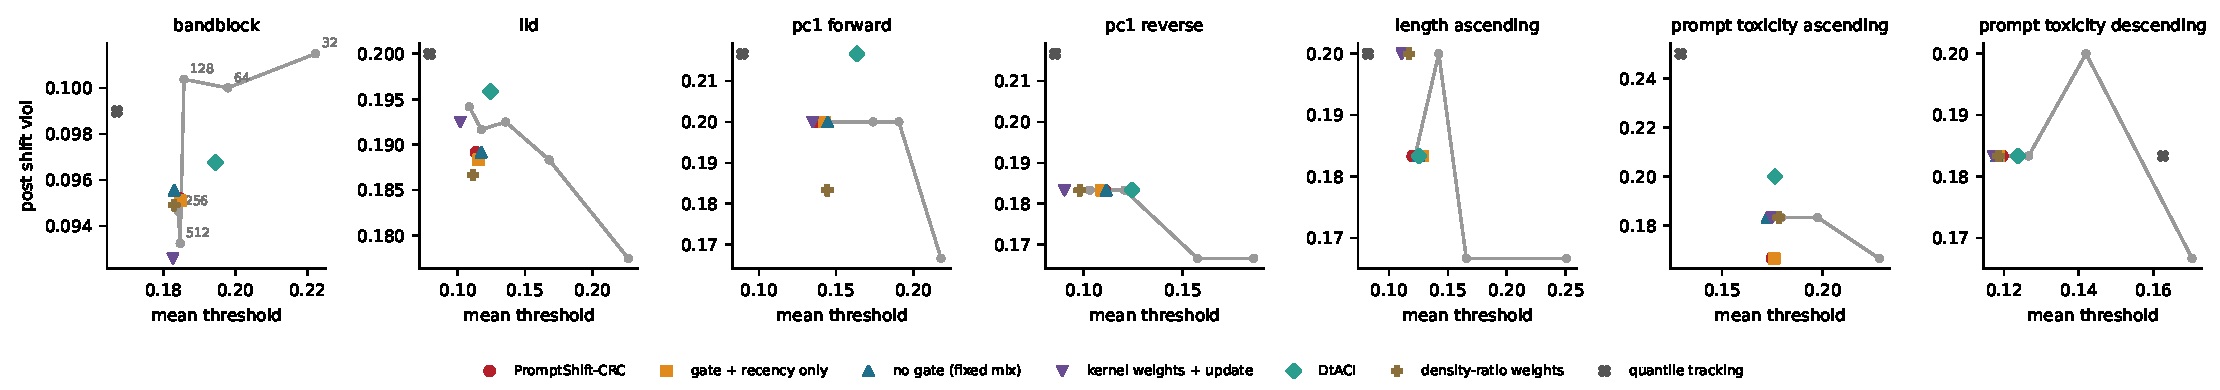
\includegraphics[width=\textwidth]{figures_v2/fig_frontier_rtp_prob.pdf}
\caption{Validity and sharpness on RealToxicityPrompts with GPT-2 continuations. Panels are ordering families (each point is the mean over the orderings in the family). The grey curve is Adaptive CRC over the window sweep; labels give the window.}
\label{fig:frontier-rtp}
\end{figure}

\subsection{Robustness to the window choice}\label{sec:res-window}

The results suggest what PromptShift-CRC offers: no window has to be chosen. The best window for Adaptive CRC depends on the stream. It is short on the synthetic streams and long on RealToxicityPrompts, and the window that is best in hindsight is known only afterwards. We state the comparison in two ways.

\emph{Rank.} Among the five Adaptive CRC windows and PromptShift-CRC, PromptShift-CRC has mean rank \regSynRank{} on the synthetic streams, \regMmluCatRank{} and \regMmluSubjRank{} on MMLU, \regRtpRank{} on RealToxicityPrompts and \regTqaRank{} on TruthfulQA (Table~\ref{tab:regret}; $1$ is the lowest violation and $3.5$ is the middle of six). It is in the better half on MMLU and RealToxicityPrompts, and not on the synthetic streams or on TruthfulQA. In every setting it is better than the worst window, by between two-fifths and two-thirds of the spread of the family.

\emph{Choosing the window elsewhere.} The best window in hindsight is selected on the data it is scored on, which biases the comparison against PromptShift-CRC. A fairer protocol chooses the window on the other families of streams and applies it to the held-out family (Table~\ref{tab:lofo}). PromptShift-CRC minus the chosen window is \lofosynthetic{} (synthetic), \lofoMMLUcategories{} and \lofoMMLUsubjects{} (MMLU), \lofoRTPbands{} (RealToxicityPrompts) and \lofoTruthfulQAcategories{} (TruthfulQA). It is lower in four of the five families. The best window changes from the shortest (synthetic) to the longest (RealToxicityPrompts), and that change is the argument for a rule that does not choose a window. We do not claim that PromptShift-CRC beats a well-chosen window; the evidence is that it avoids a poorly chosen one.

\subsection{What each component does}\label{sec:res-ablation}

On the synthetic streams and on RealToxicityPrompts the same pattern holds (Tables~\ref{tab:synthetic} and~\ref{tab:rtp_bandblock}). The online update is the component that matters most: removing it moves post-shift violation from \synPSPost{} to \synNoUpdPost{} on the synthetic streams and from \RtpPSPost{} to \RtpNoUpdPost{} on RealToxicityPrompts. The recency window with the gate is next: the variant that keeps only the gate and the recency window has post-shift violation \synGateRecPost{} (synthetic) and \RtpGateRecPost{} (RealToxicityPrompts), close to PromptShift-CRC's \synPSPost{} and \RtpPSPost{}. The kernel weights contribute least. With them alone and the update, post-shift violation is \synKernelUpdPost{} on the synthetic streams, higher than PromptShift-CRC's, with a sharper threshold. These components move post-shift violation by less than one percentage point and the mean threshold by up to $1.6$ points, and the sign depends on the stream.
